\documentclass[12pt,fleqn]{article}\usepackage{../../common}
\begin{document}

\begin{minted}[fontsize=\footnotesize]{python}
import pandas as pd
df = pd.read_csv('money.csv',parse_dates=['DATE'])
df = df[['nonfincred','inflation','DATE']]
df = df.dropna(axis=0)
df = df.set_index('DATE')
df['dcredit'] = df['nonfincred'].pct_change()*100.0
df['dinf'] = df['inflation'].pct_change()*100.0
df[['dcredit','dinf']].plot()
plt.savefig('test_01.png')
\end{minted}

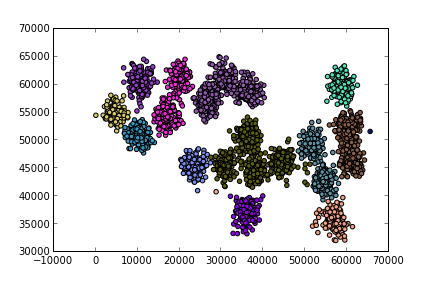
\includegraphics[height=6cm]{test_01.png}










\end{document}
